\section{Image Formation}
% 1. \textbf{Image Formation:} Capturing real-world objects into an image involves physical, geometric, and optical parameters. \\

\subsection*{Physical Parameters}
1. \textbf{Photometric:} 
   - Type, direction, and intensity of light reaching the sensor. \\
   - Surface reflectance properties. \\
2. \textbf{Geometric:} 
   - Type of projection (e.g., perspective, orthographic). \\
   - Camera pose and position. \\
3. \textbf{Optical:}
   - Lens type, focal length, aperture, and shutter speed. \\

\subsection*{Pinhole Camera Model}
1. A camera model where light passes through a pinhole onto a film/sensor. \\
- Reduces blurring by blocking most light rays and allows sharp image formation. \\

\subsection*{Projective Geometry}
1. Projection maps 3D world coordinates to 2D image coordinates. \\
   % - Example: \( u = \frac{f X}{Z} + u_0 \), \( v = \frac{f Y}{Z} + v_0 \). \\
\
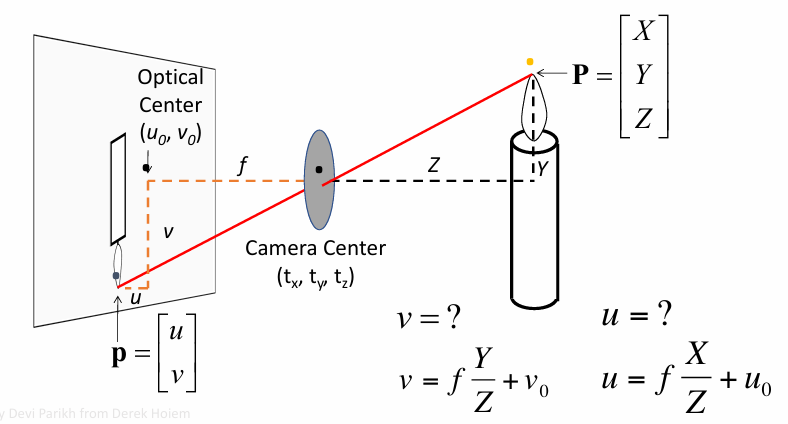
\includegraphics[width=1\linewidth]{images/l10-pinhole.png}
    % \caption{Pinhole Camera Model: Light rays from the object pass through the pinhole, forming an inverted image on the image plane.}
    % \label{fig:pinhole-model}

2. \textbf{Vanishing Points:} 3D Parallel lines -> converge at a point in the image. (Vertical vanishing point: infinity)\\
\textbf{Vanishing Line:} 3D Parallel lines -> converge at a line in the image.

\subsection*{Homogeneous Coordinates and Camera Matrix}
1. Homogeneous coordinates: add another axis, translation --> mat mul. \\
2. \textbf{Intrinsic Matrix} (\(K\)): Encodes internal camera properties. Deg of freedom: 5
   \[
   K = 
   \begin{bmatrix}
   f_x & s & c_x \\
   0 & f_y & c_y \\
   0 & 0 & 1
   \end{bmatrix}
   \]
   - \(f_x, f_y\): Focal length. \\
   - \(s\): Skew factor (usually 0) to account for non-rectangular pixels. \\
   - \(c_x, c_y\): Optical center coordinates (principal point). \\
3. \textbf{Extrinsic Matrix} (\([R | t]\)): External camera params. Deg of freedom: 6\\
   % \[
   % [R \mid t] = 
   % \begin{bmatrix}
   % R & t \\
   % 0 & 1
   % \end{bmatrix}
   % \]
   \[
   R = R_x(\alpha) R_y(\beta) R_z(\gamma)
   \]
   \[
   R_x(\alpha) = 
   \begin{bmatrix}
   1 & 0 & 0 \\
   0 & \cos \alpha & -\sin \alpha \\
   0 & \sin \alpha & \cos \alpha
   \end{bmatrix}
   % , \quad
   % R_y(\beta) = 
   % \begin{bmatrix}
   % \cos \beta & 0 & \sin \beta \\
   % 0 & 1 & 0 \\
   % -\sin \beta & 0 & \cos \beta
   % \end{bmatrix}, \quad
   % R_z(\gamma) = 
   % \begin{bmatrix}
   % \cos \gamma & -\sin \gamma & 0 \\
   % \sin \gamma & \cos \gamma & 0 \\
   % 0 & 0 & 1
   % \end{bmatrix}
   \]
   % - \(R_x(\alpha)\): Rotation around the x-axis by angle \(\alpha\). \\
   % - \(R_y(\beta)\): Rotation around the y-axis by angle \(\beta\). \\
   % - \(R_z(\gamma)\): Rotation around the z-axis by angle \(\gamma\). \\
   - \(R\), \(t\): from world's coordinate to cam's
   % - \(R\): Rotation matrix representing the camera's orientation relative to the world. \\
   % - \(t\): Translation vector representing the camera’s position. \\

\subsection*{Orthographic and Weak Perspective Proj}
1. \textbf{Orthographic Projection:} The distance to the image plane is infinite. \\
2. \textbf{Weak Perspective:} An approximation where object dimensions are small relative to the camera distance. \\

% \subsection*{Summary}
% 1. Key concepts: \textbf{vanishing points}, \textbf{pinhole camera model}, \textbf{homogeneous coordinates}. \\
% 2. Understanding these models helps explain image formation, projection, and camera calibration.
